%\documentclass[final,pdf,frames]{prosper}
\documentclass[final,pdf,darkblue,slideColor,colorBG]{prosper}
%\documentclass[final,pdf,blends]{prosper}

\usepackage[latin1]{inputenc}
\usepackage{german}
\usepackage{epsfig}

%\usepackage{graphicx}
%\DeclareGraphicsRule{.png}{bmp}{}{}

\date{8. Januar 2003}

\title{Mechatronik-Framework Projekt L�ufer}
\subtitle{Abschlussvortrag}
\slideCaption{Projekt L�ufer -- Mechatronik -- \today}

\author{Christian R�diger, Christoph Reichenbach, Markus Weimer}
\email{droso@gmx.net, jameson@linuxgames.com, markus@weimer-online.com}
\institution{Technische Universit�t Darmstadt}

%\DefaultTransition{Blinds}
\begin{document}


\maketitle

% Einleitung
\overlays{3}{%
\begin{slide}{Personen}
  \begin{itemstep}
    \item Christoph Reichenbach, Informatik, 9. Semester
    \item Christian R�diger, Informatik, 7. Semester
    \item Markus Weimer, Wirtschaftsinformatik, 7. Semester
  \end{itemstep}
\end{slide}
}

\overlays{4}{%
\begin{slide}{Umfeld: Projekt L�ufer}
\begin{itemstep}
  \item Studentisches Projekt
  \item Entwicklung eines ,,muskelgetriebenen Reisefahrzeugs''
  \item Industriepartnerschaften
  \item Innovative Technologien
\end{itemstep}
\end{slide}
}

\overlays{4}{%
\begin{slide}{Aufgabe dieser Arbeit}
\begin{itemstep}
  \item Entwicklung eines Mechatronik-Frameworks
  \item Platinen samt Mini-Betriebssystem
  \item Kommunikation
  \item Fahrer-Schnittstelle
\end{itemstep}
\end{slide}
}

\overlays{4}{%
\begin{slide}{�bersicht �ber das Folgende}
Weg einer Nachricht:
\begin{itemstep}
  \item Benutzer dr�ckt Blinker-Knopf
  \item Weg durch den PDA und die Kommunikation
  \item Umsetzung des Benutzerwunsches auf der Platine
  \item Feststellung eines Fehlers samt Benachrichtigung des Fahrers
\end{itemstep}
\end{slide}
}


% Folien von MW

\overlays{2}{%
  \begin{slide}{Das Fahrerinterface}
      \begin{minipage}{7.0cm}
        \untilSlide*{1}{%
          Gr�nde f�r einen PDA:
          \begin{itemize}
          \item Gen�gend Rechenleistung (Hochsprachen)
          \item Display (Warnhinweise)
          \item Interaktion (Einstellungen, Routing, etc.)
          \end{itemize}
        }
      \fromSlide*{2}{%
        Gr�nde f�r \emph{diesen} PDA
        \begin{itemize}
          \item Display
          \item Rechenleistung
          \item Linux (Multitasking, Programmierung)
        \end{itemize}
      }
    \end{minipage}
    \begin{minipage}{3cm}
      \begin{center}
        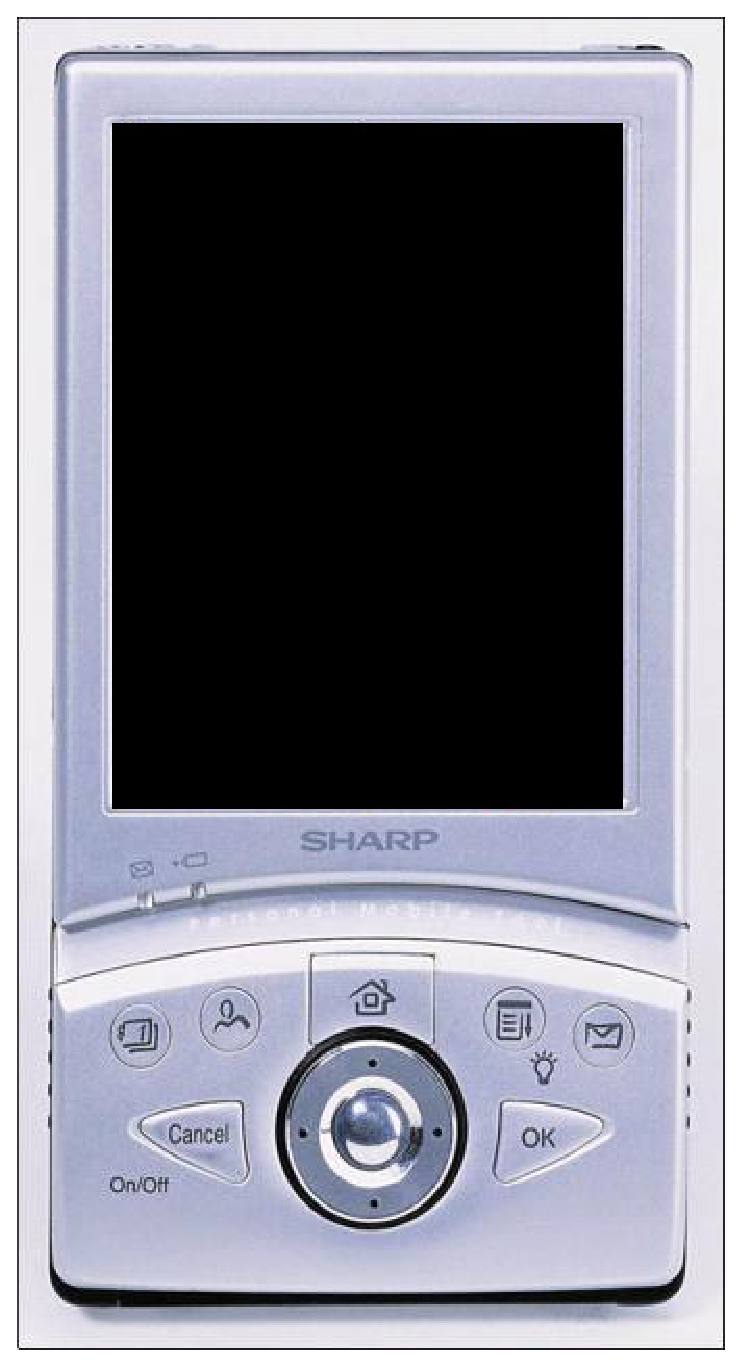
\includegraphics[width=3cm]{zaurus.eps}
      \end{center}
    \end{minipage}
  \end{slide}
}


% ============================================================


\overlays{2}{
  \begin{slide}{DPI aus Entwicklersicht}
    \untilSlide*{1}{
      \begin{center}
        Informal: Kommunizierende Automaten\\
        
\includegraphics[width=9cm, angle=-90]{zustaende.eps}

      \end{center}
    }
    \fromSlide{2}{
      Vaterklasse \texttt{Driver} f�r alle Treiber
      \begin{itemize}
      \item GUI ruft \texttt{Blinken()} des Treibers auf.
      \item \texttt{send(Message)}: Versenden von \emph{Nachrichten}.
      \item \texttt{receive(Message)}: Empfang von Nachrichten.
      \end{itemize}
    }
  \end{slide}
}


% ============================================================


  \begin{slide}{Weg der Nachricht durch das DPI}
    \begin{itemize}
    \item \texttt{Driver.send()} �berpr�ft die Nachricht
    \item \texttt{message\_dispatcher.send()} sendet auf passendem
      \texttt{bus\_manager} heraus $\to$ Indirektion
    \item \texttt{bus\_manager.send()} sendet auf passendem
      \texttt{bus} heraus $\to$ Indirektion
    \end{itemize}
  \end{slide}

% Folien Jameson
%
% Messageversand:
% Busimplementierung codiert Nachricht
% -- In LLZ-Protokoll als Datenversand (REQ)
% -- IN LLO-Protokoll als Datenversand (STX) mit Sequenzzaehler
% in seriellem Transferprotokoll
% Transfer ueber RS232C-Schnittstelle
% Decodierung auf ``Proxy''
% Unmittelbare Recodierung auf MCP2510 CAN-Controller und Transfer ueber ``dominante''
%%% CAN-Message
% Empfang der Botschaft auf allen horchenden Zielgeraeten bei explizitem Polling
% Decodierung gemaess LLO-Protokoll
% Acknowledge gemaess LLO-Protokoll fuer CAN-Bus schedulen
% Decodierung gemaess LLZ-Protokoll
% -> Ist Datenversand!
% 
%
%
%
% Rueckantwort: SX codiert Nachricht in LLZ (NTF) als Notifikation und in
%%% LLO (RTX) als Datenversand von der Peripherie
% SX versendet Nachricht, Proxy ACKnowledged
% Proxy codiert Botschaft (unueberprueft) in seriellem Transferprotokoll
% PDA empfaengt und dekodiert Botschaft in Message-Objekt

\overlays{1}{
  \begin{slide}{Codierung der Nachricht}
    \begin{minipage}{8cm}
      \begin{itemize}
      \item{Bus-Implementierung codiert Nachricht in drei Protokollschichten:
 	\begin{enumerate}
 	\item{{\bf LLZ} (Session) als \emph{Request}}
 	\item{{\bf LLO} (Transfer) als \emph{Transfer}}
 	\item{{\bf SLP} (Seriell) als \emph{Block}}
 	\end{enumerate}
      }
      \item{Versand \"uber serielle Schnittstelle an \emph{Proxy}}
      \end{itemize}
    \end{minipage}
    \begin{minipage}{2cm}
      \begin{center}
	
\includegraphics[width=3cm]{protoblock1.eps}
      \end{center}
    \end{minipage}
  \end{slide}
}

\overlays{1}{
  \begin{slide}{Nachrichtentransfer}
    \begin{itemize}
      \item{{\bf LLZ}-Protokoll
	\begin{itemize}
	  \item{Initialisierung}
	  \item{``Synchrone'' Kommunikation}
	\end{itemize}
      }
      \item{{\bf LLO}-Protokoll
	\begin{itemize}
	  \item{Ger\"ateadressierung}
	  \item{Erkennung von Fehlern}
	\end{itemize}
      }
      \item{{\bf SLP}-Protokoll
	\begin{itemize}
	  \item{Blockaufteilung f\"ur serielle Kommunikation}
	  \item{$\leftrightarrow$ Proxy-Platine (CAN-Bus-Master)}
	\end{itemize}
      }
    \end{itemize}
  \end{slide}
}

\overlays{1}{
  \begin{slide}{Nachrichtentransfer (Schema)}
    \begin{center}
      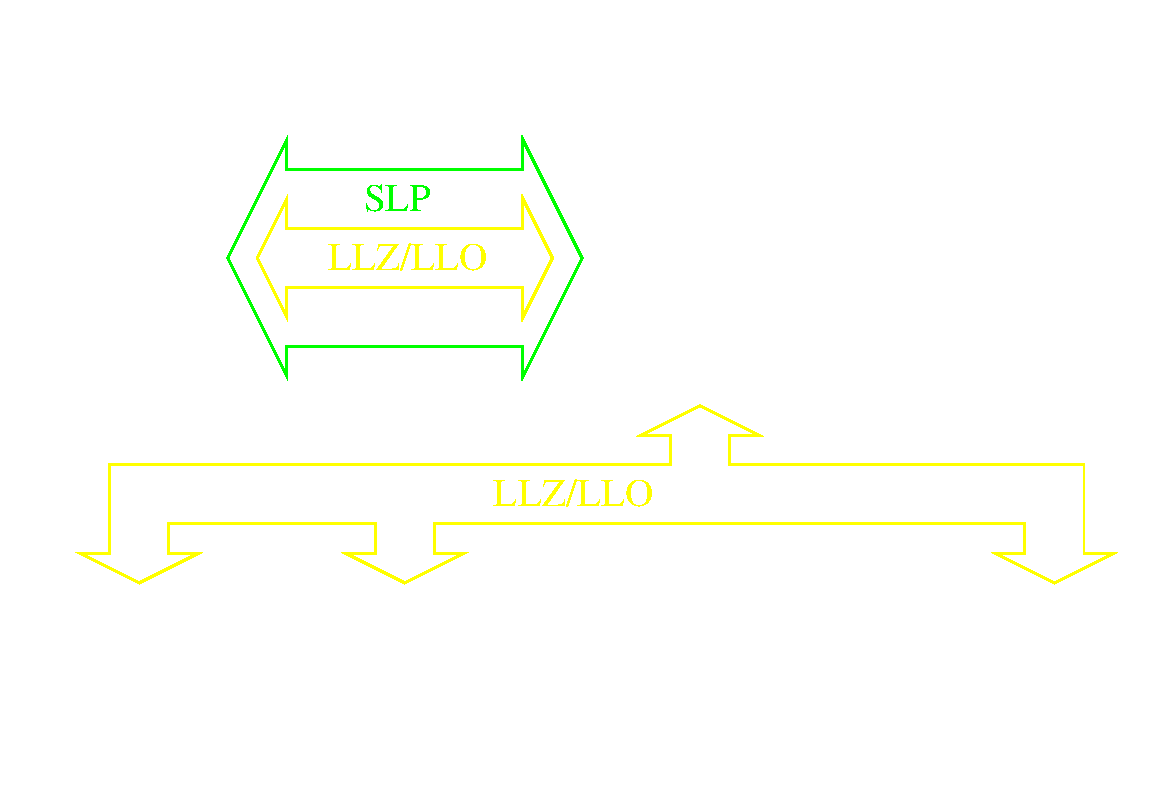
\includegraphics[width=9cm]{peripherie.eps}
    \end{center}
  \end{slide}
}



% Folien CR
\begin{slide}{Die Platine}
\begin{itemize}
  \item vom Ingenieur implementierte Logik nimmt Nachricht an
  \item Logik interpretiert Nachricht
  \item Ger�te werden mithilfe des vorgefertigten Codes ($\to$Module) instruiert
  \item unser Beispiel:
  \item die Lichtanlage soll Blinken
  \item d.h. die Low Side Switches werden �ber SPI aktiviert und geschaltet
\end{itemize}
\end{slide}


\begin{slide}{Module}
\begin{itemize}
  \item  Module sind in Macros geb�ndelte Programmteile
  \item  �ber Module ist die Peripherie erreichbar
  \begin{itemize}
  \item  Beispiel: AD-Converter, serielle Schnittstelle etc.
  \end{itemize}
  \item  Module stellen Komfort-Funktionen zu Verf�gung
  \begin{itemize}
  \item  Beispiel: Puls Weit Modulation
  \end{itemize}
\end{itemize}
\end{slide}

\begin{slide}{Module einbinden}
  \begin{itemize}
  \item Platzieren des Moduls im Programmspeicher:\newline
  \begin{verbatim}
org 400
SPI_CODE_SEG
  \end{verbatim}
  \item Aufruf einer darin definierten Routine
   \begin{verbatim}
	MOV	W, # SPI_TLE2
	CALL 	@SPI_select_device
	CALL	@SPI_TLE_SO_SI
  \end{verbatim}
  \end{itemize}
\end{slide}



%\overlays{6}{
%\begin{slide}{Das Programm als Automat}
%  \onlySlide*{1}{\includegraphics[width=8cm]{Automat2.eps}}
%  \onlySlide*{2}{\includegraphics[width=8cm]{Automat3.eps}}
%  \onlySlide*{3}{\includegraphics[width=8cm]{Automat4.eps}}
%  \onlySlide*{4}{\includegraphics[width=8cm]{Automat5.eps}} 
%  \onlySlide*{5}{\includegraphics[width=8cm]{Automat6.eps}}
%  \onlySlide*{6}{\includegraphics[width=8cm]{Automat7.eps}}
%\end{slide}
%}


\begin{slide}{Im Kontext Mechatronik}
\begin{center}
        
\includegraphics[width=8cm]{Mechatronik_sys.eps}
\end{center}
\end{slide}



  \begin{slide}{Sicherheit}
     % \begin{minipage}{6.0cm}
	Die Sicherheit liegt in der Hand des Ingenieurs\newline
	Ein Beispiel wie es sein k�nnte:
          \begin{itemize}
          \item ADC stellt zu niedrigen oder hohen Stromfluss fest
          \item �bergang in failsafe mode, der alle Ger�te ''abschaltet''
          \item Abgabe einer Warnmeldung an CAN Bus
          \end{itemize}
    %\end{minipage}
    %\begin{minipage}{4cm}
     % \begin{center}
      %  \includegraphics[width=4cm]{LightAutomaton.eps}
      %\end{center}
    %\end{minipage}
  \end{slide}










% Folien Jameson
\overlays{1}{
  \begin{slide}{R\"uckversand}
    \begin{itemize}
      \item{Codierung in {\bf LLZ}/{\bf LLO}}
      \item{Versand \"uber CAN mit nachrichtenspezifischer Priorit\"at
	\begin{itemize}
	\item{Transfer bei expliziter Busfreigabe des Masters (in regelm\"a\ss igen Intervallen)}
	\item{Acknowledge direkt von Proxy}
	\end{itemize}
      }
      \item{Serieller Versand an PDA
	\begin{itemize}
	\item{Codierung in {\bf SLP}}
	\end{itemize}
      }
    \end{itemize}
  \end{slide}
}


\overlays{1}{
  \begin{slide}{Fehlerbehandlung}
    \begin{itemize}
    \item{Bitfehler von CAN erkannt}
    \item{Regelm\"a\ss ige Keep-Alives, sonst Selbstabschaltung der Peripherie}
    \item{{\bf LLO}: Explizite Acknowledgements}
    \item{PDA $\rightarrow$ Peripherie
      \begin{itemize}
      \item{Entkopplung durch Sequenzz\"ahler}
      \end{itemize}
    }
    \item{Peripherie $\rightarrow$ PDA
      \begin{itemize}
      \item{Nachrichten werden unmittelbar von Proxy best\"atigt}
      \end{itemize}
    }
    \end{itemize}
  \end{slide}
}


% Folien MW

\begin{slide}{R�ckweg der Nachricht}
  \begin{itemize}
  \item Die Nachricht kommt als \texttt{Message} beim
    \texttt{message\_dispatcher} an.
  \item �berpr�fung der Nachricht (ID, Befehl)
  \item �bergabe an Treiber �ber \texttt{receive()}
  \item Reaktion des Treibers.
  \end{itemize}
\end{slide}


% ============================================================


\overlays{3}{%
  \begin{slide}{Kommunikation mit der GUI}
    \untilSlide*{2}{
      Verwendung von Signals und Slots aus QT
      \begin{itemize}
      \item Treiber definiert seine Signale.
      \item GUI verbindet Signale mit Slots von GUI-Elementen,
        Methoden, anderen Treibern etc.
      \item $\to$ Fahrzeuglogik wird durch Routing der Signale
        implementiert.
      \end{itemize}
      \OnlySlide{2} Drawback: Festlegung auf QT und Pr�prozessor.
    }
    \fromSlide*{2}{
      Hier: 
      \begin{itemize}
      \item Treiber wirft Signal \texttt{birne\_defekt}
      \item GUI verbindet dies mit Warnelement auf Display
      \end{itemize}
    }
  \end{slide}
  
}

% Abschluss
\begin{slide}{Fazit -- Was haben wir gelernt }
\begin{itemize}
\item Interdisziplin�res Arbeiten
\item Technik:
  \begin{itemize}
  \item Elektrotechnik
  \item Protokolldesign f�r Mikrocontroller
  \item Linux auf ,,kleinen'' Rechnern
  \end{itemize}
\item Public Relations (Messen, Sponsoren, etc.)
\item Arbeit internationaler OpenSource Gruppen
\end{itemize}
\end{slide}

% ============================================================


\begin{slide}{Ausblick}
  Konkret:
  \begin{itemize}
    \item Entwicklung der Motorsteuerung mit aktueller Implementierung
    \item Ab 15.5.: Fertigstellung des Frameworks
  \end{itemize}
%
  Ideen f�r Alternativen:
%
  \begin{itemize}
    \item Hochsprachenf�hige Platine
    \item Definitionssystem bzw. -Sprache f�r Zust�nde
    \item $\to$ Code-Generator $\to$ Automatische Kommunikation
  \end{itemize}
\end{slide}



\end{document}
